\documentclass{beamer}

\usepackage{beamerthemesplit, joyce-beamer}

\newcommand{\vsep}{\vspace{0.2cm}}

\title{The Normal Approximation of the Binomial
  Distribution} 
\author{Joyce Tipping} 
\date{Wednesday, November 19, 2008}

\begin{document}
\frame{\titlepage}

\frame{
\frametitle{Why?}

When $n$ gets large, the binomial probabilities become
difficult to calculate.
}

\frame{ 
\frametitle{\textit{Very} Quick Review} 
\textbf{Random Variable:} A function that assigns a
probability to each possible outcome.

\vsep
\pause

\textbf{Expected Value:} The long-run expected outcome of a
random variable.

\vsep
\pause

\textbf{Variance:} A measurement of the spread of a random variable.
}

\frame{
\frametitle{The Bernoulli}
A Bernoulli experiment has the following properties:
\begin{enumerate}
\item One trial
\item Two outcomes: Success or Failure
\item Known probability of success
\end{enumerate}
}


\frame{
\frametitle{The Binomial}
A binomial experiment has the following properties:
\begin{enumerate}
\item n trials, where n is known
\item The trials are independent
\item Each trial has two outcomes: Success or Failure
\item Probability of success is known and fixed
\end{enumerate}
}

\frame{
\frametitle{The Binomial}
A binomial experiment can be thought of as a sum of
independent Bernoulli trials.
}

\frame{
\frametitle{The Central Limit Theorem}

Let $X_1, \ldots, X_n$ be a random sample from a
distribution with mean $\mu$ and variance $\sigma^2 <
\infty$. Then,
\begin{equation*}
  \frac{\overline X - \mu}{\frac{\sigma}{\sqrt{n}}}
\end{equation*}
approaches the standard normal, $Z \sim N(0,1)$ as $n
\rightarrow \infty$.
}

\frame{
\frametitle{The Central Limit Theorem}

\begin{equation*}
  \frac{\overline X - \mu}{\frac{\sigma}{\sqrt{n}}}
\end{equation*}

\vsep

\begin{equation*}
  = \quad \frac{\frac{1}{n} \displaystyle \sum_{i=1}^{n} X_i -
  \mu}{\frac{\sigma}{\sqrt{n}}}
\end{equation*}

\vsep

\begin{equation*}
  = \quad \frac{\displaystyle \sum_{i=1}^{n} X_i - n\mu}{\sqrt{n} \;
    \sigma}
\end{equation*}
}

\frame{
\frametitle{The Central Limit Theorem}

Let $X_1, \ldots, X_n$ be a random sample from a
distribution with mean $\mu$ and variance $\sigma^2 <
\infty$. Then,
\begin{equation*}
  \frac{\displaystyle \sum_{i=1}^{n} X_i - n\mu}{\sqrt{n} \;
    \sigma}
\end{equation*}
approaches the standard normal, $Z \sim N(0,1)$, as $n
\rightarrow \infty$.
}

\frame{
\frametitle{The Approximation}

Let $X_i \sim Ber(p)$. \par
$\mu_x = p$ \par
$\sigma^2_x = pq$ $\longrightarrow$ $\sigma_x = \sqrt{pq}$

\pause
\vspace{1cm}

Then, we have $\displaystyle \sum_{i=1}^{n} X_i \sim bin(n,
p)$.

\vsep

Therefore, by the CLT, $bin(n,p)$ is approximately normal
with
\begin{align*}
  &\mu = n \cdot \mu_x = np \\
  &\sigma = \sqrt{n} \cdot \sigma_x = \sqrt{npq}
\end{align*}
whenever $n$ is large.
}

\frame{
\frametitle{Example}
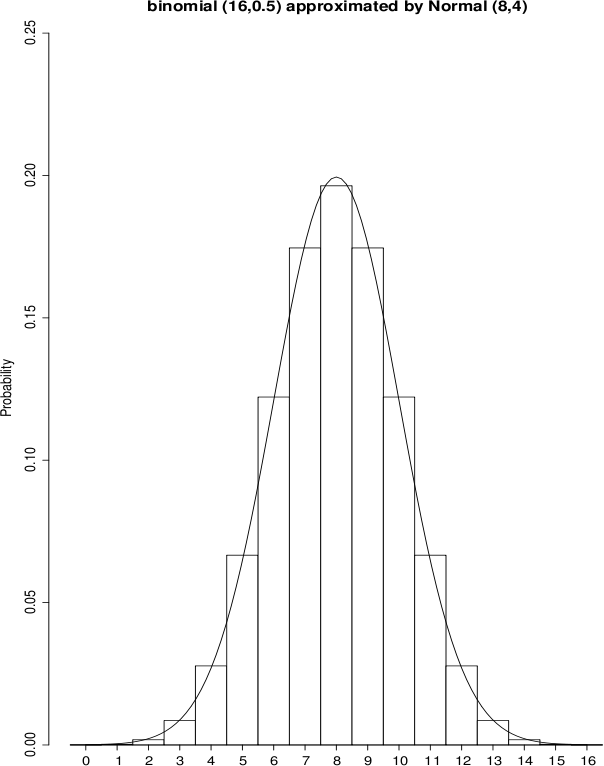
\includegraphics[height=3in]{binomial-approximated-with-normal.png}
}

\frame{
\frametitle{When It Works}

The normal approximation works well when the binomial is
symmetric:
\begin{enumerate}
\item $p$ is close to 0.5 \quad {\sc or}
\item $n$ is very large
\end{enumerate}

\vsep

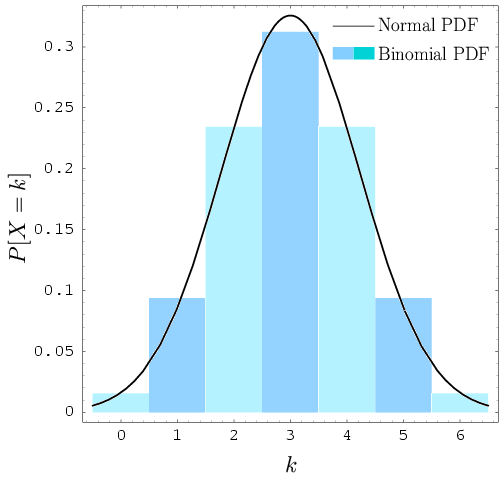
\includegraphics[height=2in]{binomial-centered.png}
}

\frame{
\frametitle{Coming Up Soon ...}

When $p$ is not close to 0.5 and $n$ is not large, the
binomial is skewed.

\vsep

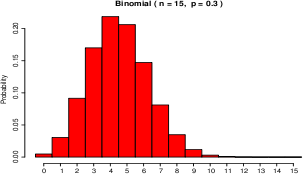
\includegraphics[height=1in]{binomial-skewed.png}

\vsep

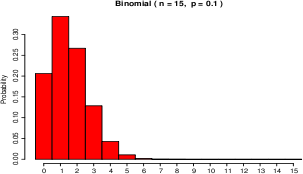
\includegraphics[height=1in]{binomial-very-skewed.png}

\vsep

In this case, the skew-normal is a better approximation.
}

\end{document}